\documentclass{beamer}
\usepackage[utf8]{inputenc}
\usepackage{xurl}

\usetheme{Madrid}
\usecolortheme{default}


\title[LFS]
{Linux From Scratch}

\subtitle{Estoy aburrido}

\author[Ludway]
{Ludwig Alvarado}


\date[2024]
{2024}

\logo{
\includegraphics[height=1.2cm]{img/Tux.png}}


\begin{document}


\frame{\titlepage}

\begin{frame}
  \frametitle{¿Quién soy?}
  \begin{columns}
    \column{0.5\textwidth}
    \begin{itemize}
      \item 19 años.
      \item Estudiante de doble titulación en Ingeniería de Sistemas y Ciencia de Datos.
      \item Fanático del Software Libre y su comunidad.
      \item GitHub: \url{www.github.com/theludway}
    \end{itemize}
    \column{0.5\textwidth}
    \begin{figure}
      \centering
      
\includegraphics[width=0.8\textwidth]{img/Yo.jpg}
    \end{figure}
  \end{columns}
\end{frame}

\begin{frame}
  \frametitle{Objetivos}
  \begin{columns}
    \column{0.5\textwidth}
    \begin{itemize}
      \item Aprender más sobre los programas que componen GNU/Linux.
      \item Obtener una versión de Linux From Scratch para luego ser llevada a Beyond Linux From Scratch.
      \item Documentar el proceso realizado.
    \end{itemize}

    \column{0.5\textwidth}
    \begin{figure}
      \centering
      
\includegraphics[width=0.8\textwidth]{img/gnu-tux.jpg}
    \end{figure}
  \end{columns}

\end{frame}

\begin{frame}
  \frametitle{¿Por qué lo hago?}
  \begin{columns}
    \column{0.5\textwidth}
    \begin{itemize}
      \item Curiosidad.
      \item Quiero aprender más.
      \item Mucho tiempo libre (desempleado).
    \end{itemize}

    \column{0.5\textwidth}
    \begin{figure}
      \centering
      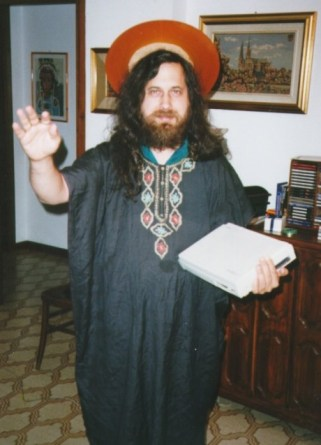
\includegraphics[width=0.6\textwidth]{img/saintignucius.jpg}
    \end{figure}
  \end{columns}

\end{frame}

\begin{frame}
  \frametitle{Herramientas}
  \begin{itemize}
    \item YouTube.
    \item LaTeX.
    \item OBS.
    \item Virtual Machine Manager.
    \item Fedora 41.
    \item Foros de comunidad.
    \item ChatGPT.
    \item Libro LFS.
    \item GIMP.
  \end{itemize}

\end{frame}

\begin{frame}
  \frametitle{Licencia}
  \begin{columns}
    \column{0.5\textwidth}
    \begin{itemize}
      \item YouTube y GitHub.
      \item Creative Commons CC BY 4.0
    \end{itemize}

    \column{0.5\textwidth}
    \begin{figure}
      \centering
      
\includegraphics[width=\textwidth]{img/CC.png}
    \end{figure}
  \end{columns}

\end{frame}




\end{document}
